% !TEX root = ../main.tex
\section{Hold-up-problemet}\label{thr:hold-up-problem}

\paragraph{Definisjon.} \emph{Hold-up} oppstår når en part har foretatt en \emph{relasjonsspesifikk investering} (aktiva med lav alternativverdi), og motparten utnytter den resulterende forhandlingsmakten til å reforhandle vilkårene ex post. Konsekvensen er \emph{underinvestering} ex ante fordi den investerende parten forutser ekspropriering av \emph{quasi-renter}. [SLIDE]

\subsection*{Forklaring}

BSZ kap.\ 19 og Williamson (1979, 1985) beskriver hold-up som det sentrale kontraktproblemet ved outsourcing med spesifikke investeringer. [SLIDE/BOK]

\textbf{Mekanisme:}
\begin{enumerate}\setlength{\itemsep}{2pt}
\item Leverandør $S$ investerer $I$ i spesialtilpasset produksjonsutstyr for kunde $B$. Utstyret er verdt $V$ for $B$, men bare $V_0 \ll V$ i alternativ bruk (\emph{asset specificity}).
\item \emph{Quasi-rente} $= V - V_0$ er den ekstra verdien som skapes av relasjonen. Den er approprierbar fordi $S$ er locked in etter investering.
\item $B$ vet dette og reforhandler prisen ned mot $V_0$ etter at $S$ har investert -- $S$ må akseptere fordi $V_0$ er den eneste exit-opsjonen.
\item \emph{Ex ante-konsekvens:} $S$ forutser hold-up og underinvesterer (investerer mindre enn sosialt optimalt), eller krever safeguards.
\end{enumerate}

\textbf{Typer asset specificity} (Williamson):
\begin{itemize}\setlength{\itemsep}{1pt}
\item \textbf{Site specificity:} Geografisk samlokalisering (raffineri ved oljebrønn).
\item \textbf{Physical asset specificity:} Spesialtilpasset utstyr/verktøy (bilpresser til én modell).
\item \textbf{Human asset specificity:} Spesifikk kompetanse/opplæring som ikke er overførbar.
\item \textbf{Dedicated assets:} Kapasitetsinvestering kun for én kundes volum.
\item \textbf{Temporal specificity:} Timing er kritisk; forsinkelse ødelegger verdien (ferskvarer, JIT).
\end{itemize}

\textbf{Løsninger:}
\begin{itemize}\setlength{\itemsep}{2pt}
\item \textbf{Vertikal integrasjon} -- eliminerer hold-up ved å forene eierskap. Eier av begge ledd har ingen insentiv til å holde seg selv opp. [SLIDE]
\item \textbf{Langsiktige kontrakter} med detaljerte prisklausuler, volum-forpliktelser og penalty-klausuler. Men kontrakten kan ikke dekke alt (\thref{costly-contracting}{costly contracting}). [BOK]
\item \textbf{Felles eierskap av aktiva} (joint venture) -- deler residuell kontrollrett.
\item \textbf{Kryssholding og gjensidig avhengighet} -- begge parter investerer spesifikt og holder hverandre ``gissel'' (\emph{mutual hostage}).
\item \textbf{Reputasjon} i repeterte spill -- hold-up ødelegger fremtidige gevinster.
\end{itemize}

\subsection*{Kjerneforutsetninger}
\begin{itemize}
\item Investeringen er relasjonsspesifikk (lav $V_0$ relativt til $V$).
\item Kontrakten kan ikke fullt spesifisere ex post-vilkår (\thref{costly-contracting}{costly contracting}).
\item Reforhandling er mulig -- ingen mekanisme hindrer opportunistisk krav.
\item Minst én part må investere \emph{før} den andre leverer sin del.
\end{itemize}

\subsection*{Muligheter}
\begin{itemize}
\item Forklarer vertikal integrasjon som svar på spesifikke investeringer.
\item Predikerer underinvestering i leverandørrelasjoner uten safeguards.
\item Forklarer kontraktsdesign: penalty-klausuler, escrow, step-in-rettigheter.
\item Forklarer hvorfor noen bransjer er mer vertikalt integrert (høy asset specificity) enn andre.
\end{itemize}

\subsection*{Begrensninger og kritikk}
\begin{itemize}
\item Forutsetter at motparten er fullt opportunistisk -- i praksis demper reputasjon og tillit hold-up.
\item Integrasjon løser hold-up men skaper \thref{agency-costs}{agency costs} internt -- trade-off.
\item Modellen er binær (invest/don't invest); i praksis er graden av spesifisitet et kontinuum.
\item Empirisk: vanskelig å separere hold-up fra andre motiver for integrasjon.
\end{itemize}

\subsection*{Modell / illustrasjon}

\begin{center}
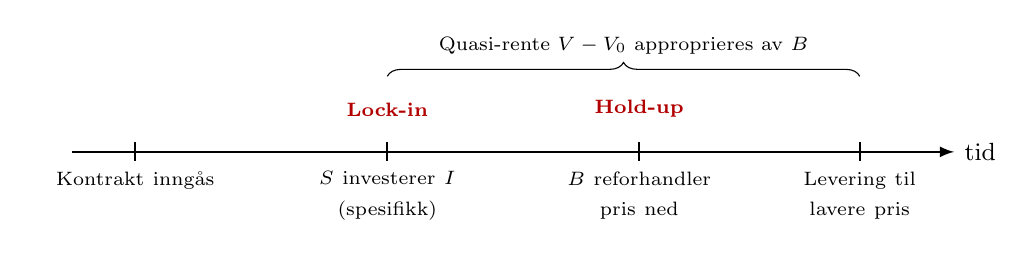
\begin{tikzpicture}[>=latex, scale=0.8, every node/.style={font=\small}]
  % Tidslinje
  \draw[->, thick] (0,0) -- (14,0) node[right] {tid};
  % Events
  \draw[thick] (1,0.15) -- (1,-0.15) node[below, text width=2.5cm, align=center] {\scriptsize Kontrakt inngås};
  \draw[thick] (5,0.15) -- (5,-0.15) node[below, text width=2.5cm, align=center] {\scriptsize $S$ investerer $I$\\(spesifikk)};
  \draw[thick] (9,0.15) -- (9,-0.15) node[below, text width=2.5cm, align=center] {\scriptsize $B$ reforhandler\\pris ned};
  \draw[thick] (12.5,0.15) -- (12.5,-0.15) node[below, text width=2.5cm, align=center] {\scriptsize Levering til\\lavere pris};
  % Labels above
  \node[above, red!70!black, font=\bfseries\scriptsize] at (5,0.4) {Lock-in};
  \node[above, red!70!black, font=\bfseries\scriptsize] at (9,0.4) {Hold-up};
  % Quasi-rent brace
  \draw[decorate, decoration={brace, amplitude=5pt}] (5,1.2) -- (12.5,1.2);
  \node[above] at (8.75,1.4) {\scriptsize Quasi-rente $V - V_0$ approprieres av $B$};
\end{tikzpicture}
\end{center}
\textit{Figur: Tidslinjen for hold-up. Etter spesifikk investering er $S$ locked in; $B$ utnytter dette ved reforhandling. [BOK]}

\subsection*{Eksempler}
\begin{itemize}\setlength{\itemsep}{2pt}
\item \textbf{GM--Fisher Body (1920-tallet):} Fisher Body investerte i pressverktøy spesifikt for GM-karosserier. Da etterspørselen steg, forsøkte Fisher å utnytte GMs avhengighet. GM løste hold-up ved å kjøpe Fisher Body (vertikal integrasjon). Klassisk eksempel i Williamson-litteraturen. [EKS]
\item \textbf{Intel og PC-produsenter:} Intel investerer lite relasjons\-spesifikt -- prosessorer er standardiserte. Lav asset specificity $\Rightarrow$ outsourcing fungerer. Kontrast til Fisher Body. [EKS]
\item \textbf{Mærsk og skipsverft (Hyundai Heavy):} Spesialdesignede containerskip representerer site-/physical-specificity. Mærsk sikrer seg med detaljerte kontrakter, milestone-betalinger og inspeksjonsrett -- kontraktuell safeguard i stedet for integrasjon. [CASE]
\end{itemize}

\subsection*{Kobling til søyle og andre teorier}
Søyle: \SOne\ (eierskap som allokering av residuell kontrollrett) og \SThree\ (insentiver til relasjonsspesifikk investering). Relaterte: \thref{vertical-integration-outsourcing}{Vertikal integrasjon og outsourcing}, \thref{boundaries-of-the-firm}{Boundaries of the Firm}, \thref{costly-contracting}{Costly contracting}, \thref{specific-vs-general-knowledge}{Spesifik vs.\ generell viden}, \thref{agency-costs}{Agency costs}.

\paragraph{Brukt i spørsmål:} Q12 (primært), Q11 (referert).
